\newpage
\subsection{Factorial}
En muchas ocasiones, para poder obtener un resultado principal, es necesario el
c\'alculo secundario del factorial de un n\'umero muy grande, resultando en una
limitante computacional. Un ejemplo de esto es el teorema de \textit{Chebichev}.

La f\'ormula Stirling, nombrada así en honor al matem\'atico escoc\'es del siglo
XVIII James Stirling, es una aproximaci\'on para el c\'alculo del factorial de
un n\'umero muy grande y dif\'icil de computar con la definici\'on est\'andar.

La aproximaci\'on de Stirling dice lo siguiente:
\begin{eqnarray}
	n!\approx \sqrt{2\pi n}(\frac{n}{e})^n\\
	n!\approx \sqrt{2\pi n} (n^n)(e^{-n})
	\label{stirling}
\end{eqnarray}

La Ec. \eqref{stirling} permite una forma r\'apida de calcular el factorial.
Aunque el error va disminuyendo de forma exponencial conforme crece el n\'umero,
existe una mejor aproximaci\'on que involucra un t\'ermino m\'as.


\begin{equation}
	n!\approx \sqrt{2\pi n}(\frac{n}{e})^n(1+\frac{1}{12n})
	\label{Stirling}
\end{equation}
\begin{figure}[h!]
	\centering
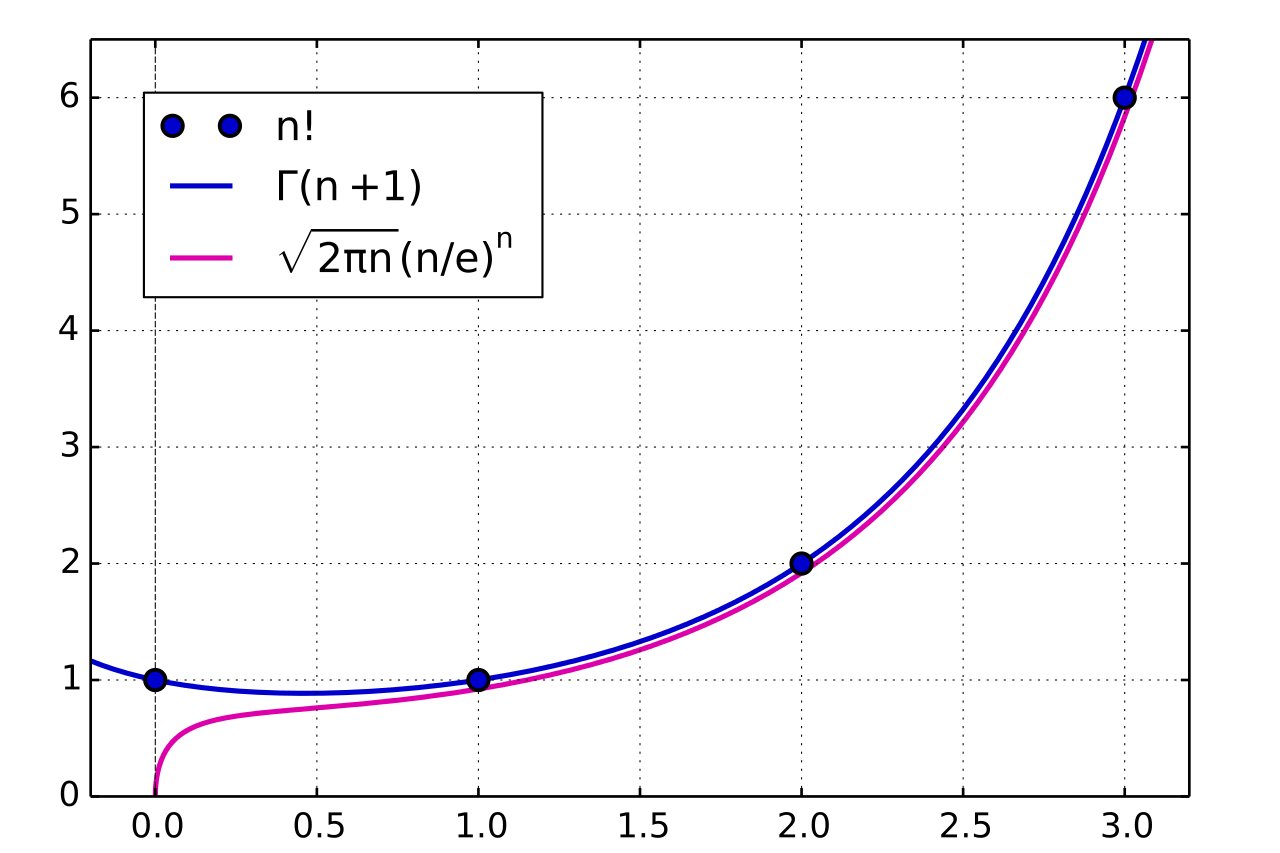
\includegraphics[scale=0.30]{figures/factorial_gamma_stirling.png}
\caption{Error de aproximaci\'on stirling respecto del factorial.}
\label{stirling_error}
\end{figure}

\pagebreak
\subsection{Código para realizar la aproximación de Stirling}
\lstinputlisting[language=Python]{../src/stirling.py}

